\documentclass[12pt]{article}
\usepackage[utf8]{inputenc}
\usepackage[russian]{babel}
\usepackage{indentfirst}
\usepackage{graphicx} % отображение картинок
\usepackage{subfigure}
\usepackage{amssymb} % отображение математической нотации
\usepackage[normalem]{ulem} % для подчеркиваний \uline
\usepackage[nottoc,notlot,notlof]{tocbibind} % для отображения списка литературы в содержании
\ULdepth = 0.20em % расстояние от линии до текста
\usepackage[
    left=30mm, right=20mm,
    top=20mm, bottom=20mm,
    bindingoffset=0mm
    ]{geometry} % настройка границ документа



\begin{document}

    \begin{titlepage}
        \begin{center}
            \textsc{
            \large
            МОСКОВСКИЙ ГОСУДАРСТВЕННЫЙ УНИВЕРСИТЕТ \\
            имени М.В. Ломоносова
            } \\
            [5mm]

            Факультет Вычислительной Математики и Кибернетики \\
            Кафедра Интелектуальных Информационных Технологий \\
            Лаборатория Технологий Программирования 
            \vfill
    
            \textsc{Курсовая работа} \\
            по теме: \\
            [5mm]
            {\LARGE
            <<Динамическая аутентификация пользователей \\
            на основе анализа работы с компьютерной мышью>>
            }
            \vfill
            \begin{flushright}
                \textsc{Березникер Алексей Витальевич} \\
                3 курс, группа 320 \\
                [5mm]
                Научный руководитель: \\
                к.ф.-м.н. Казачук Мария Андреевна \\
            \end{flushright}
            \vfill

            Москва, 2020 г.
        \end{center}
    \end{titlepage}



    \tableofcontents
    \newpage



    \section{Аннотация}
    \label{sec:Annotation}

    \par Целью данной работы является исследование существующих и разработка собственных алгоритмов динамической аутентификации пользователя на основе анализа работы с компьютерной мышью, показывающих высокое качество работы и способных работать в динамическом режиме. \\
    \par Мы фокусируемся на независимой от контекста системе динамической аутентификации, которая реагирует на каждое отдельное действие, выполненное пользователем. \\
    \par Отметим, что динамическая аутентификация не является альтернативным решением безопасности для первоначального входа в систему, она обеспечивает дополнительную меру безопасности наряду с первоначальным логином.

    \newpage



    \section{Введение}
    \label{sec:Intro}
    
    \subsection{Область применения}
    \label{sec:Intro:ApplicationArea}
    
    \par В настоящее время неотъемлемой частью различных сфер деятельности человека стало использование информационных систем. Огромное количество информации ограниченного доступа переносится, хранится и обрабатывается в информационных системах, что формирует потребность в обеспечении их защищенности. \\
    \par Люди используют механизмы контроля доступа, такие как пароль, магнитные карты или биометрию, для защиты от несанкционированного доступа другого человека. Это означает, что пользователь должен предоставить подтверждение своей личности при запуске или разблокировке системы. Однако во многих случаях люди оставляют компьютер без присмотра, чтобы попить чашку кофе, пойти и поговорить с коллегой, или просто потому, что у них нет привычки выключать компьютер. \\
    \par Контроль доступа к компьютеру обычно реализуется как единоразовое подтверждение личности во время начальной процедуры входа в систему. Предполагается, что в течении всего сеанса в системе будет находиться зарегистрированный пользователь. К сожалению, когда компьютер оставлен без присмотра, любой человек может получить доступ к тем же источникам, что и подлинный пользователь. \\
    \par Защита информации в информационных системах обеспечивается созданием комплексной системы защиты, одной из главных составляющих которой являются методы защиты от несанкционированного доступа. \\
    \par Основой программно-технических средств защиты от несанкционированного доступа являются процедуры идентификации и аутентификации пользователей. Идентификатором служит уникальный признак объекта, позволяющий отличить его от других объектов. А под процедурой аутентификации подразумевается процесс проверки принадлежности субъекту доступа предъявленного им идентификатора. \\


    \subsection{Методы аутентификации}
    \label{sec:Intro:ApplicationArea:AuthenticationMethods}

    \par Существующие методы осуществления аутентификации можно разделить на три категории. К первой относятся методы, основанные на обладании субъекта аутентификации некоторым секретным знанием. В качестве такого знания может выступать секретное слово, пароль или цифровой сертификат. Данный метод является самым распространенным и простым. Он часто подвержен атакам со стороны злоумышленников. \\
    \par Ко второй категории относятся методы, основанные на наличии у субъекта идентификации некоторого физического объекта. Таким объектом может быть, например, ключ, флеш-накопитель или магнитная карта. Аутентификация по предъявлении чего-либо, чем владеет пользователь, имеет сходные недостатки, и, кроме того, добавляется риск передачи, утери, кражи или копирования ключа. А также требуется специальное оборудование для распознавания предмета, используемого при аутентификации. \\
    \par К последней категории относят методы, основанные на собственных свойствах субъекта доступа. В качестве таких свойств могут рассматриваться биометрические данные пользователя, т.е. уникальные биологические и физиологические характеристики, которые позволяют установить личность человека. Методы аутентификации, основанные на проверке подлинности через предъявление биометрического образа называется биометрической аутентификацией. \\

    \subsubsection{Методы биометрической аутентификации}
    \label{sec:Intro:ApplicationArea:AuthenticationMethods:Biometric}

    \par Существующие в настоящее время методы биометрической аутентификации разделяются на два класса:
    \begin{enumerate}
        \item \textbf{Статические методы биометрической аутентификации}, \\
        основанные на физиологических характеристиках человека, находящиеся при нём в течение всей его жизни. Например, проверка отпечатка пальца, сетчатки глаза или геометрии лица. Статическая аутентификация заключается в эпизодической проверке личности пользователя (например, при его входе в систему), после чего пользователь может свободно пользоваться системой.
        \item \textbf{Динамические методы биометрической аутентификации}, \\
        основанные на поведенческих характеристиках человека. Анализ голоса, клавиатурного почерка или работы с компьютерной мышью. Динамическая аутентификация предполагает проведение проверки личности пользователя постоянно на протяжении всей сессии.
    \end{enumerate}

    \par Основным недостатком методов проверки пользователей, основанных на физиологической биометрии, является то, что они требуют аппаратные устройства, такие как датчики отпечатков пальцев и сканеры сетчатки, которые дороги и не всегда доступны. Хотя проверка отпечатков пальцев становится широко распространенной в ноутбуках, она все еще недостаточно популярна и не может быть использована в веб-приложениях. Кроме того, отпечатки пальцев могут быть скопированы.В свою очередь методы, основанные на поведенческой биометрии не требуют специальное оборудование, так как они используют обычные устройства, такие как мышь и клавиатура. \\
    \par Другим важным отличием между физиологической и поведенческой биометрией является временной аспект. Поведенческая биометрия может отличаться в зависимости от режима работы пользователя и времени суток, когда она была зафиксированна. Это усложняет процесс подражания для обхода системы, даже в случае перехватывата данных.\\

    \par Очевидно, динамическая аутентификация пользователей является предпочтительной, так как она исключает сценарии, при которых злоумышленник получает доступ к информационной системе после того, как легитимный пользователь прошел процедуру аутентификацию.

    \newpage



    \section{Актуальность}
    \label{sec:Relevance}

    \par Таким образом, мы видим проблему отсутствия контроля факта смены пользователя и компрометации идентификаторов, которую мы предлагаем решить использованием биометрических характеристик пользователя для динамической аутентификации. \\
    \par Достоинство нашего подхода заключается в простоте внедрения: нужно лишь устройство ввода (компьютерная мышь) и специальное программное обеспечение, позволяющее проводить анализ.

    \newpage



    \section{Постановка задачи}
    \label{sec:FormulationOfProblem}
    
    \par Задачей данной работы является исследование существующих и разработка собственных алгоритмов динамической аутентификации пользователя на основе анализа работы с компьютерной мышью, показывающих высокое качество работы и способных работать в динамическом режиме. \\
    \par Наше решение должно выполнять задачи незаметно для пользователя, выявлять злоумышленника как можно быстрее, в то же время избегая в максимально возможной степени неправильной блокировки легитимного пользователя.

    \newpage



    \section{Обзор существующих решений}
    \label{sec:Overview}

    \subsection{Цели обзора}
    \label{sec:Overview:Goals}

    \begin{enumerate}
        \item Выявить достоинства и недостатки существующих подходов;
        \item Выявить наиболее релевантные признаки для построения модели пользователя;
        \item Выявить методы построения модели, показывающие наилучшее качество работы;
        \item Найти набор данных в открытом доступе для проведения собственных исследований;
        \item Сформулировать направления дальнейших исследований.
    \end{enumerate}

    \newpage


    \subsection{Показатели эффективности}
    \label{sec:Overview:Metrics}

    \par Согласно [TODO] и [TODO], Решение об аутентификации должно основываться на результате процесса сопоставления вновь представленных биометрических данных с предварительно сохраненными эталонными шаблонами. \\

    \noident\textsc{Коэффициент ложных отклонений} \\
    Коэффициент ложных отклонений (FRR: False Rejection Rate) - это доля случаев, когда биометрическая система не предоставляет доступ легитимному пользователю. В статистическом смысле, FRR - это ошибка I рода. FRR также известен как частота ложных несовпадений (FNMR: False Non Match Rate). \\

    \noident\textsc{Коэффициент ложного принятия} \\
    \noident Биометрическая безопасность использует коэффициент ложного принятия (FAR: False Acceptance Rate) для доли случаев, когда система предоставляет доступ неуполномоченному лицу. С точки зрения статистики, FAR - это ошибка II рода. Этот коэффициент также известен как частота ложных совпадений (FMR: False Match Rate). \\

    \noident\textsc{Равный коэффициент ошибок} \\
    \noident Одним из способов обобщить рабочие характеристики биометрической системы безопасности является рассмотрение коэффициента переходных ошибок (CER: Crossover Error Rate), также известного как равный коэффициент ошибок (EER: Equal Error Rate). Это коэффициент, при котором ошибки FAR и FRR равны. EER дает возможность сравнивать системы. Чем меньше EER, тем лучше. Меньшее значение EER означает, что можно настроить систему так, чтобы частота ошибок как для I рода, так и для II рода была меньше. \\

    \par В приложениях безопасности FAR (неавторизованный доступ) хуже, чем FRR (блокировка авторизованного пользователя). Первое может стать катастрофой, а второе - неудобством. Конечно, может быть контекст, в котором последствия FAR и FRR равны или что FRR хуже, но обычно это не так. \\

    \begin{figure}[h]
        \centering
        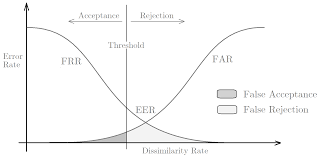
\includegraphics{EER.png}
        \caption{Графическая интерпретация FAR, FRR и EER}
        \label{sec:Overview:Metrics:fig:EER}
    \end{figure}
    \vspace{10mm}

    \noident\textsc{Рабочая характеристика системы} \\
    \noident Рабочая характеристика системы (ROC: Receiver operating characteristic) или ROC-кривая - это график компромисса между характеристиками FAR и FRR. В общем случае алгоритм принимает решение на основе порогового значения, которое определяет, насколько близко к эталону должен быть вход, чтобы его можно было считать совпадающим. Если порог уменьшится, будет меньше ложных отклонений, но больше ложных принятий. И наоборот, более высокий порог уменьшит FAR, но увеличит FRR. Качество оценивают как площадь под ROC кривой (ROC AUC: area under ROC curve).

    \begin{figure}[hb]
        \centering
        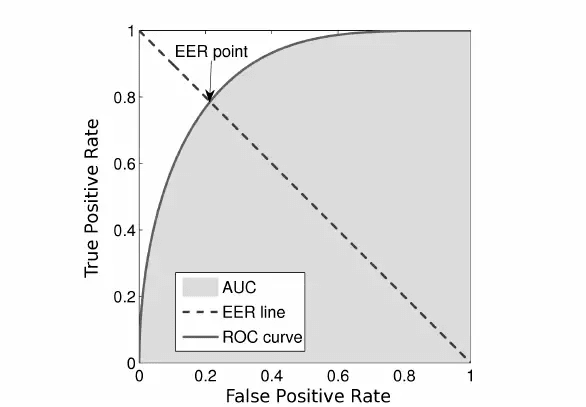
\includegraphics[width=0.75\linewidth]{EER_ROC.png}
        \caption{Связь между EER и ROC-curve}
        \label{sec:Overview:Metrics:fig:EER}
    \end{figure}

    Кроме того авторы [TODO] верно заметили, что для системы на самом деле важно знать не только об обнаружении нарушителя, но и когда было совершено внедрение, т.е. сколько действий нарушитель был в состоянии совершить до обнаружения. Поэтому они предложили использовать следующие характеристики для оценки эффективности работы системы: \\

    \noident\textsc{Среднее количество действий самозванца} \\
    Среднее количество действия самозванца (ANIA: Average Number of Imposter Actions) показывает сколько успеет совершить нарушитель до того момента, как он будет заблокирован системой. \\

    \noident\textsc{Среднее количество подлинных действий} \\
    Среднее количество подлинных действий (ANGA: Average Number of Genuine Actions) характеризует количество действий авторизованного пользователя до его ошибочной блокировки системой. \\

    В данных терминах система будет обладать лучшими качествами при минимизации ANIA и максимизации ANGA.


    \subsection{Построение признакового пространства}
    \label{sec:Overview:Features}
    
    \begin{table}[h]
        \centering
        \tiny
        \renewcommand{\arraystretch}{3.0}
        \renewcommand{\tabcolsep}{2mm}
        \begin{tabular}{ || l | c || l | c ||}
            \hline
            {\normalsize Признак & \normalsize Формула &  \normalsize Признак & \normalsize Формула} \\ [5mm] \hline
            Direction bin & Divided into 8 bins (45º) & Curve acceleration & $\frac{Curvespeed}{\Delta t}$ \\ \hline
            Actual distance & $\sqrt{(x_n-x_0)^2 + (y_n-y_0)^2}$ & Mean movement offset & $\frac{1}{n} \sum_{i=1}^{n} det(...) / norm(P_n - P_0)$ \\ \hline
            Actual distance bin & Divided into 20 bins & Mean movement error & $\frac{1}{n} \sum_{i=1}^{n} \left|det(...) / norm(P_n - P_0)\right|$ \\ \hline
            Curve length & $\frac{1}{n} \sum_{i=1}^{n-1} \sqrt{(x_i-x_{i+1})^2 + (y_i-y_{i+1})^2}$ & Mean movement variability & $\sqrt{\sum_{i=1}^{n} \frac{(y_i - movementoffset)^2}{n-2}}$ \\ \hline
            Curve length bin & Divided into 20 bins & Mean curvature & $\frac{1}{n} \sum_{i=0}^{n} \frac{\angle P(x_i, y_i)P(0,0)P(x_i, 0)}{\sqrt{x_{i}^2 + y_{i}^2}}$ \\ \hline
            Length ration & $\frac{Curvelength}{Actualdistance}$ & Mean curvature change ratio & $\frac{1}{n} \sum_{i=0}^{n} \frac{\angle P(x_i, y_i)P(0,0)P(x_i, 0)}{\sqrt{(x_n-x_i)^2 + (y_n-y_i)^2}}$ \\ \hline
            Actual speed & $\frac{Actualdistance}{\Delta t}$ & Mean curvature velocity & $\frac{Meancurvature}{\Delta t}$ \\ \hline
            Curve speed & $\frac{1}{n} \sum_{i=0}^{n-1} \frac{\sqrt{(x_i-x_{i+1})^2 + (y_i-y_{i+1})^2}}{t_{i+1} - t_i}$ & Mean angular velocity & $\frac{1}{n} \sum_{i=0}^{n-2} \frac{\angle P_i P_{i+1} P_{i+2}}{t_{i+2} - t_i}$ \\ \hline
        \end{tabular}
        \caption{Признаковое пространство}
        \label{sec:Overview:Features:table:FeaturesFormulas}
    \end{table}
    
    ...
    
    \begin{itemize}
        \item Траектория центра масс (TCM: Trajectory Center of Mass)
        $$
        TCM = \frac{1}{S_{n-1}} \sum_{i=1}^{n-1} t_{i+1} \sqrt{(x_{i+1} - x_{i})^2 + (y_{i+1} - y_i)^2}
        $$
        \item Коэффициент рассеивания (SC: Scattering Coefficient)
        $$
        SC = \frac{1}{S_{n-1}} \sum_{i=1}^{n-1} t_{i+1}^2 \sqrt{(x_{i+1} - x_{i})^2 + (y_{i+1} - y_i)^2} - TCM^2
        $$
        \item Третий момент ($M_3$)
        $$
        M_3 = \frac{1}{S_{n-1}} \sum_{i=1}^{n-1} t_{i+1}^3 \sqrt{(x_{i+1} - x_{i})^2 + (y_{i+1} - y_i)^2}
        $$
        \item Четвертый момент ($M_4$)
        $$
        M_4 = \frac{1}{S_{n-1}} \sum_{i=1}^{n-1} t_{i+1}^4 \sqrt{(x_{i+1} - x_{i})^2 + (y_{i+1} - y_i)^2}
        $$
        \item Траектория кривой (TCrv: Trajectory Curvature)
        $$
        TCrv = \frac{\dot{x}\ddot{y} - \ddot{x}\dot{y}}{(\dot{x}^2 + \dot{y}^2)^\frac{3}{2}}
        $$
        \item Кривизна скорости (VCrv: Velocity Curvature)
        $$
        VCrv = \frac{\ddot{v}}{(1 + \dot{v}^2)^\frac{3}{2}}
        $$
    \end{itemize}

    \newpage



    \section{Исследование и построение решения задачи}
    \label{sec:Research}
    
    \subsection{Сбор данных и извлечение признаков}
    \label{sec:Research:Data}

    \subsubsection{Описание наборов данных}
    \label{sec:Research:Data:Description}
    
    \par По своей сущности данные могут отличаться числом пользователей, принявших участие в эксперименте, размером собранной информации, и, что самое важное, средой сбора. Среда может быть:
    \begin{itemize}
        \item \textsc{контролируемой}: пользователь выполняет строго поставленные задачи. Например, кликает на появляющиеся на экране объекты или работает только с текстовым форматом данных (тогда будет преобладать состояние прокрутки колесика компьютерной мыши);
        \item \textsc{неконтролируемой}: пользователь работает в привычной для него обстановке и выполняет повседневные для своей деятельности задачи.
    \end{itemize}
    \par Очевидно, что для расширения области применения нашей системы необходимо для обучения использовать данные, собранные в неконтролируемой среде. \\
    \par По итогам обзора было собрано 3 набора данных для оценки производительности поведенческих биометрических алгоритмов на основе динамики работы с компьютерной мышью в целях аутентификации пользователя. \\
    
    \noindent\textsc{BALABIT} \cite{BALABIT} \\
    \noident Это датасет, предоставленный компанией BalaBit IT Security, специализируещейся на разработке программного обеспечения и сервисов для информационной безопасности, в 2016 году в рамках одноименного конкурса Balabit Mouse Dynamics Challenge. Набор данных доступен для исследователей и экспертов в области IT-безопасности и науки, используется в большинстве научных статей обзора. Данные собраны в неконтролируемой среде и включают информацию о времени и позиционировании указателя мыши. В эксперименте приняло участие 10 человек. В среднем для обучения мы имеем 43 $\pm$ 17 часов работы для каждого пользователя. \\
    
    \noindent\textsc{TWOS} \cite{TWOS} \\
    \noident Этот датасет был собран во время конкурса, организованного Сингапурским университетом технологии и дизайна в марте 2017 года. Набор данных содержит действия 24 пользователей, которые собирались в неконтролируемой среде в течение 5 дней. Однако информация о взаимодейсвтии с компьютерной мышью есть только для 4 пользователей. В среднем мы имеем ?? $\pm$ ?? часов работы для каждого пользователя. \\
    
    \noindent\textsc{DATAIIT} \\
    \noident Датасет, собранные на нашей кафедре в рамках исследования задачи динамической аутентификации пользователя. Данные собраны в неконтролируемой среде. В эксперименте приняло участие 20 человек. В среднем мы имеем 21 $\pm$ 5 часов работы для каждого пользователя. \\


    \subsubsection{Структура данных}
    \label{sec:Research:Data:Struct}
    
    \par Набор данных состоит из тренировочной и тестовой части в соотношении 4 к 1. Каждая часть содержит в себе записи о легитимных сеансах всех пользователей из множества $\mathfrak{U}=\{U_1, \ldots, U_j, \ldots, U_q\}$. Работа пользователя разбита на сессии разной продолжительности $U_j = \{S_1, \ldots, S_i, \ldots, S_m\}$ с записями вида $S_i = \text{(time, xpos, ypos)}$. \\
    \par Далее каждую сессию мы разбиваем на сегменты с ограничением по временному порогу сверху и по минимальному количеству действий в этот промежуток времени снизу. По полученному сегменту строится один вектор признаков. \\
    \par Графическая визуализация структуры данных представлена на Рис.~\ref{sec:Research:Data:Description:fig:DataStructure}

    \begin{figure}[h]
        \centering
        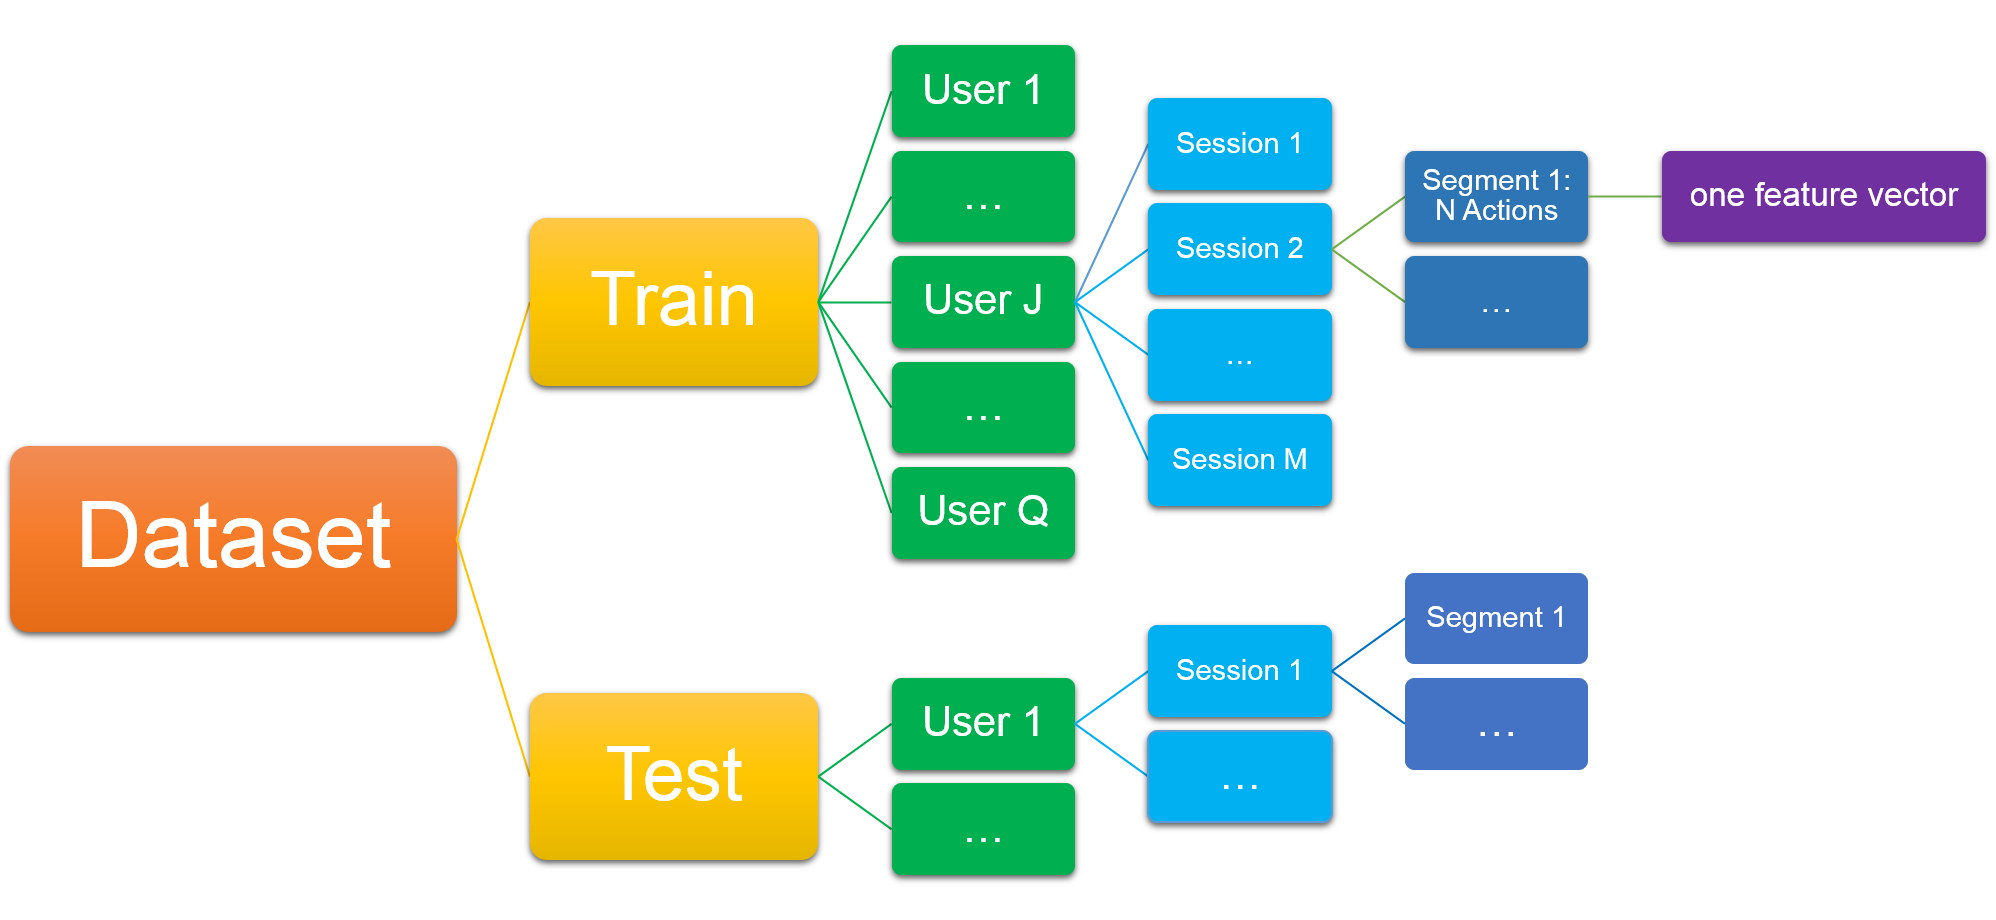
\includegraphics[width=\linewidth]{DataStructure.png}
        \caption{Структура данных}
        \label{sec:Research:Data:Description:fig:DataStructure}
    \end{figure}


    \subsubsection{Выявленные особенности данных}
    \label{sec:Research:Data:Features}
    
    Во время анализа данных были обнаружены следующие особенности:
    \begin{enumerate}
        \item Полностью дублирующиеся записи в таблице;
        \item Дубликаты временных меток;
        \item Множественные дубликаты положения мыши (зацикливание);
        \item Сверхбольшие значения координат;
        \item В датасете BALABIT:
        \begin{enumerate}
            \item В состоянии прокрутки колеса (Scroll) положение мыши перемещается в начало координат;
            \item Основная работа пользователей происходит в левом нижнем углу экрана.
        \end{enumerate}
    \end{enumerate}

    
    \subsection{Построение признакового пространства}
    \label{sec:Research:FeatureSpace}


    \subsection{Построение модели пользователя}
    \label{sec:Research:Model}
    
    \subsubsection{Задача поиска аномалий}
    \label{sec:Research:Model:Anomaly}

    \par Согласно \cite{Dyakonov, NoveltyDetection}, в анализе данных есть два направления, которые занимаются поиском аномалий: детектирование выбросов (Outlier Detection) и детектирование новизны (Novelty Detection). Как и выброс «новый объект» — это объект, который отличается по своим свойствам от объектов обучающей выборки. Но в отличие от выброса, его в самой выборке пока нет. Задачей обнаружения новизны является идентификация новых или неизвестных данных, о которых система не знает во время обучения. \\
    \par Например, при анализе замеров температуры и отбрасывании аномально больших или маленьких значений, происходит борьба с выбросами. А при создании алгоритма, который для каждого нового замера оценивает, насколько он похож на предыдущие, и выбрасывает аномальные — детектирование новизны.


    \subsubsection{OneClassSVM}
    \label{sec:Research:Model:OneClassSVM}

    \par Метод опорных векторов (SVM: Support Vector Machine) - это семейство мощного статистического обучения методов классификации и регрессии. Они доказали свою эффективность во многих практических применениях. SVM основывается на индуктивном принципе минимизации структурных рисков (SRM: Structural Risk Minimization). \\
    \par Одноклассовый метод опорных векторов (OC-SVM: One Class SVM) был предложен, как расширение SVM, для выявления новизны или выбросов в наборах данных. Важную роль OC-SVM играет в области обнаружения вторжений. \\
    \par Основная идея алгоритма заключается в поиске геперплоскости в признаковом пространстве, которая максимально отдаляет данные от начала координат

    \begin{figure}[h]
        \centering
        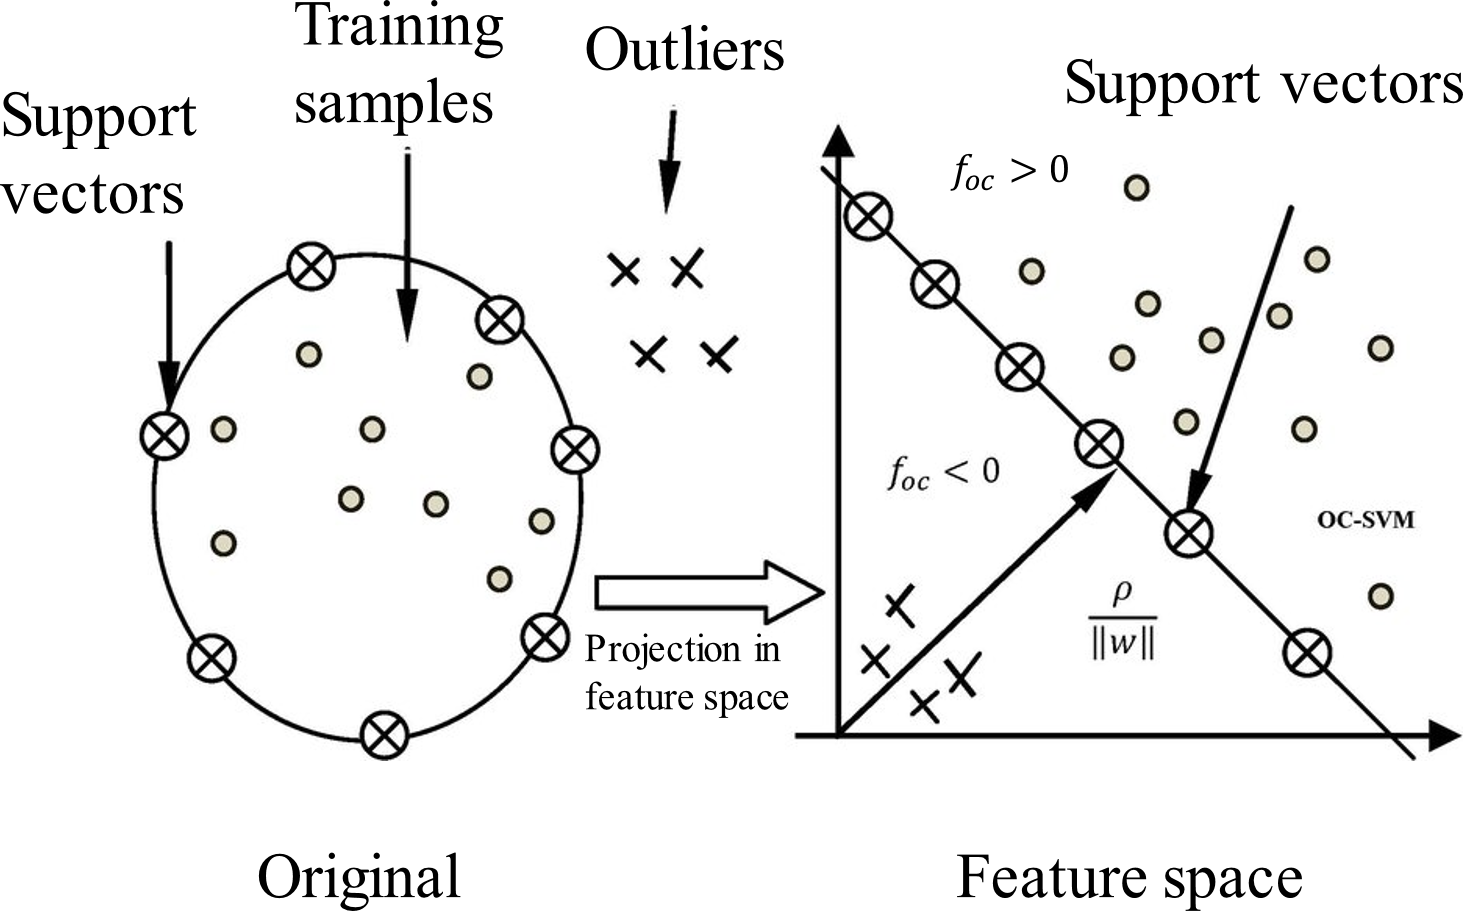
\includegraphics[width=0.6\linewidth]{OneClassSVM.png}
        \caption{Одноклассовый метод опорных векторов}
        \label{sec:Research:Model:OneClassSVM:fig:OneClassSVM}
    \end{figure}
    

    \subsubsection{IsolationForest}
    \label{sec:Research:Model:IsolationForest}
    
    \par Изоляционный лес (IF: Isolation Forest), как и любой другой метод ансамбля деревьев, построен на основе деревьев решений (DT: Decision Tree). Алгоритм обучения строит ансамбль изоляционных деревьев на основе рекурсивной и рандомизированной процедуры структурированного разбиения: сначала случайным образом выбирается объект, а затем выбирается случайное значение между минимальным и максимальным значением выбранного объекта. \\
    \par Выбросов в данных не много и, зачастую, они находятся дальше от обычных наблюдений в пространстве признаков. Вот почему при использовании такого случайного разбиения они должны быть идентифицированы ближе к корню дерева.В случае аномальных наблюдений необходимо меньше расщиплений.
    
    \begin{figure}[h]
        \centering
        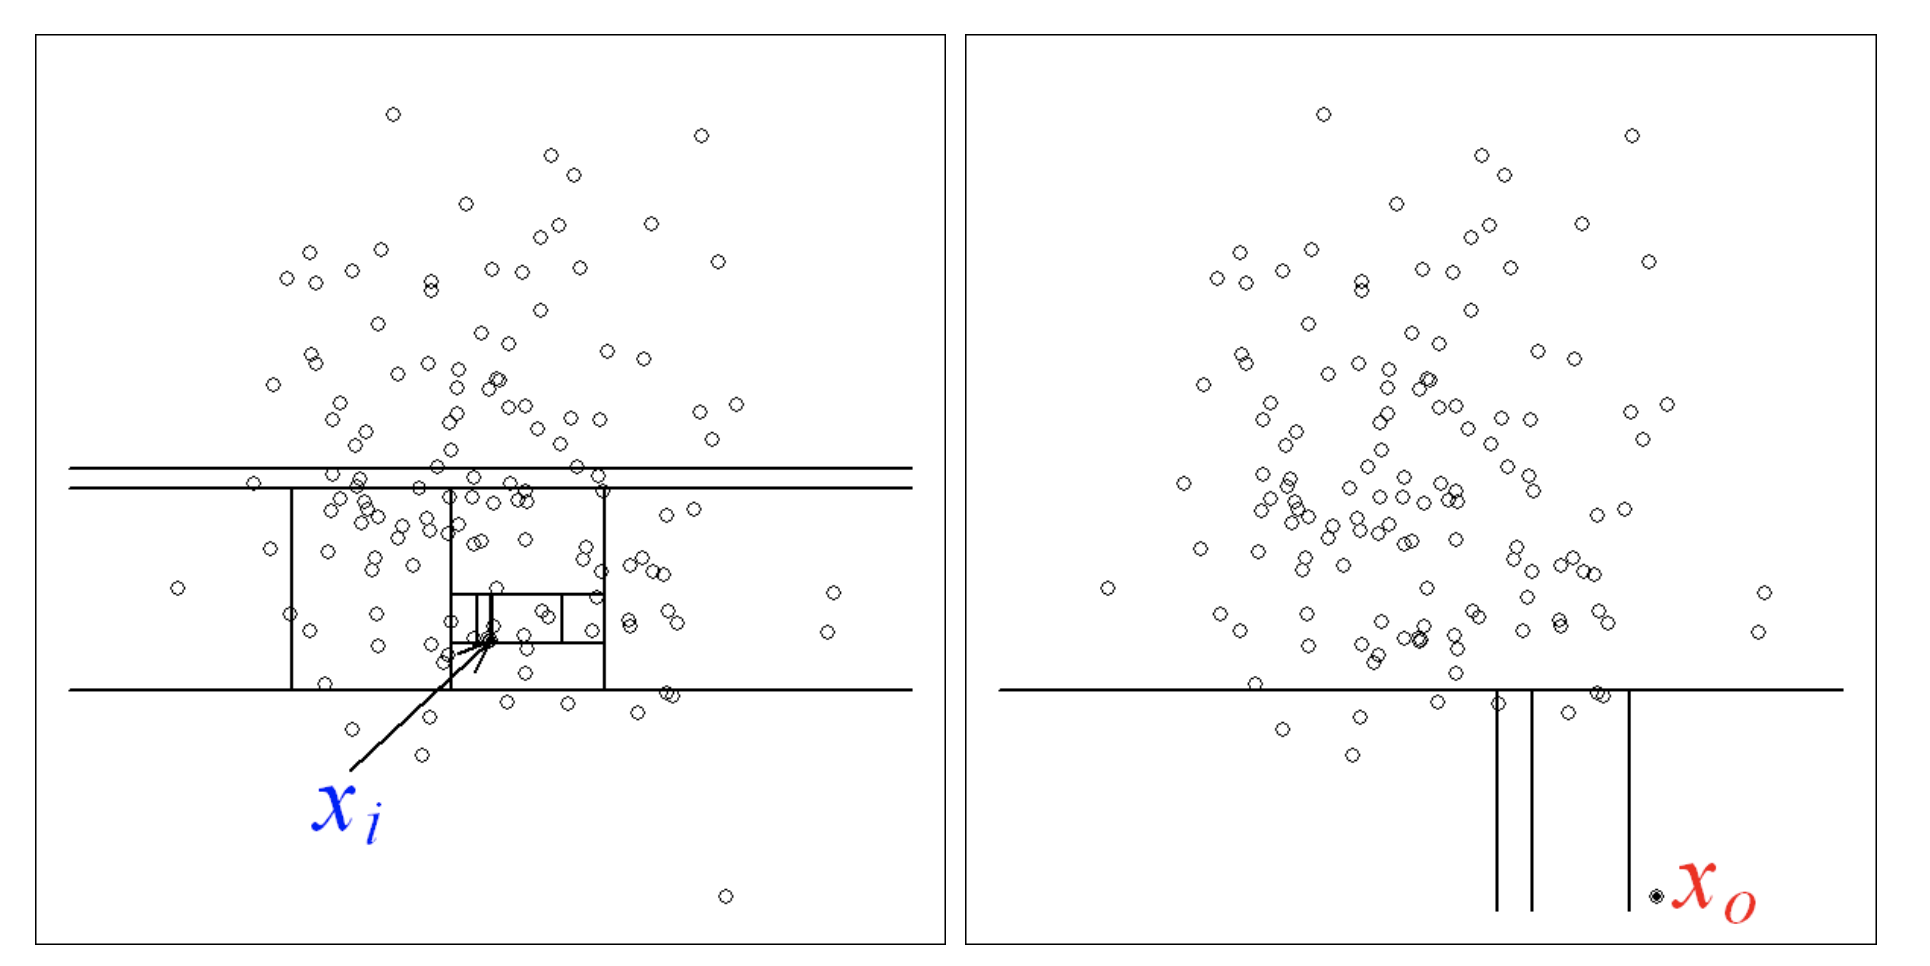
\includegraphics[width=0.8\linewidth]{IsolationForest.png}
        \caption{Определение нормальных и аномальных наблюдений}
        \label{sec:Research:Model:IsolationForest:fig:IsolationForest}
    \end{figure}
    
    \par Так, на Рис.~\ref{sec:Research:Model:IsolationForest:fig:IsolationForest} синим цветом показано нормальное наблюдение $x_i$, а красным - аномальное $x_0$. Здесь аномальная точка была разделена в несколько шагов, в то время как для изоляции нормального наблюдения потребовалось больше разделений.\\
    
    \par Для принятия решения об аномальности наблюдения алгоритм используют следующую функцию:
    $$
    S(x,n) = 2^{-\frac{E(h(x))}{c(n)}}
    $$
    \noident где $h(x)$ - длина пути наблюдения $x$ , $c(n)$ - средняя длина пути неудачного поиска в бинарном дереве поиска, а $n$ - количество внешних узлов. \\

    \par Каждое наблюдение получает индекс аномальности, на основе которого принимается решение:
    \begin{itemize}
        \item Оценка, близкая к 1, указывает на аномальность наблюдения
        \item Оценка, близкая к 0, указывает на нормальное поведение наблюдения
    \end{itemize}

    \subsubsection{EllipticEnvelope}
    \label{sec:Research:Model:EllipticEnvelope}

    \par Эллипсоидальная аппроксимация данных (EE: Elliptic Envelope) - ковариационная оценка, предполагающая, что данные имеют распределение Гаусса. Ограничивающий контур имеют эллиптическую форму. Любые данные за пределами эллипса классифицируются как аномальные. \\

    \par Рассмотрим метод подробнее. Процедура EE использует алгоритм FAST-Minimum Covariance Determinate для оценки размера и формы эллипса. Данный алгоритм выбирает неперекрывающиеся подвыборки данных и вычисляет среднее значение $\mu$ и ковариационную матрицу $C$ в признаковом пространстве для каждой подвыборки. Расстояние Махаланобиса $dMH$, вычисляется для каждого многомерного вектора данных (признака) $x$ в каждой подвыборке, по формуле:
    $$
    dMH = \sqrt{(x-\mu)^T C (x-\mu)}
    $$
    \noident и затем данные упорядочивают по возрастанию $dMH$. Эта процедура повторяется до сходимости определителя матрицы ковариации. Ковариационная матрица с наименьшим определителем из всех подвыборок образует эллипс, который охватывает часть исходных данных. Данные в пределах поверхность эллипса считаются нормальными, а вне эллипс - аномальными.

    \subsubsection{LocalOutlierFactor}
    \label{sec:Research:Model:LocalOutlierFactor}

    Локальный уровень выброса (LOF: Local Outlier Factor)

    \subsubsection{Визуализация работы методов}
    \label{sec:Research:Model:Visualization}

    Посмотрим на работу описанных методов. Для этого сформируем двумерный набор тестовых данных, содержащий 100 объектов, 5\% из которых будут выбросами. Первый набор данных (a) будет состоять из одного кластера, второй (b) - из трёх, а последний набор (c) - из десяти, что позволит сильнее разнести объекты в пространстве.

    % features
    \begin{figure}[h!]
        \centering
        \subfigure[]{
            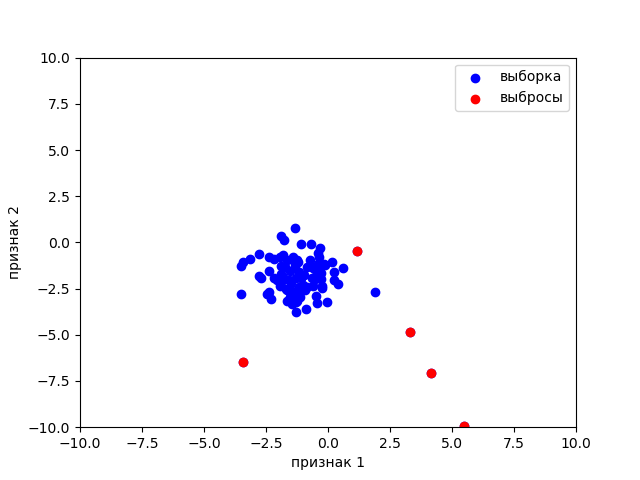
\includegraphics[width=0.3\linewidth]{features_1.png}
            \label{sec:Research:Model:Visualization:fig:featueres:1}
        }
        \subfigure[]{
            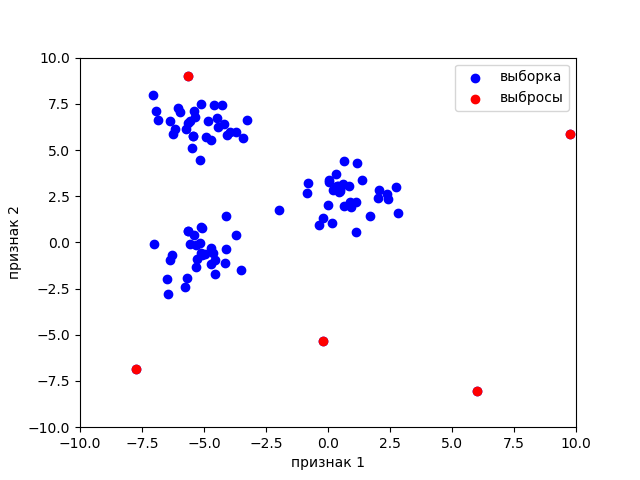
\includegraphics[width=0.3\linewidth]{features_3.png}
            \label{sec:Research:Model:Visualization:fig:featueres:3}
        }
        \subfigure[]{
            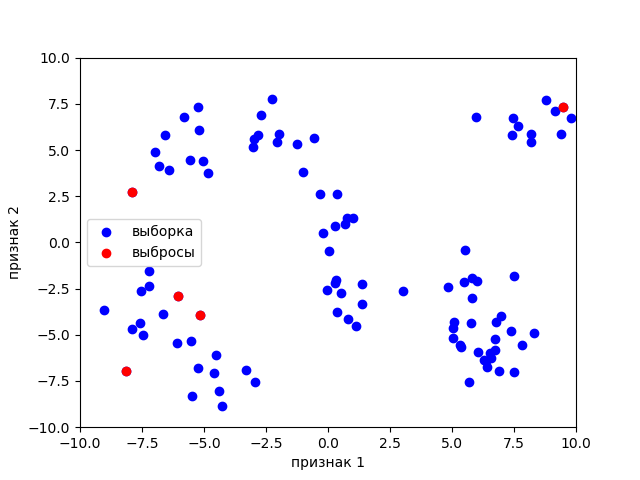
\includegraphics[width=0.3\linewidth]{features_10.png}
            \label{sec:Research:Model:Visualization:fig:featueres:10}
        }  
        \caption{ТОДО \subref{sec:Research:Model:Visualization:fig:featueres:1} }
        \label{sec:Research:Model:Visualization:fig:featueres}
    \end{figure}

    % OneClassSVM
    \begin{figure}[h!]
        \centering
        \subfigure[]{
            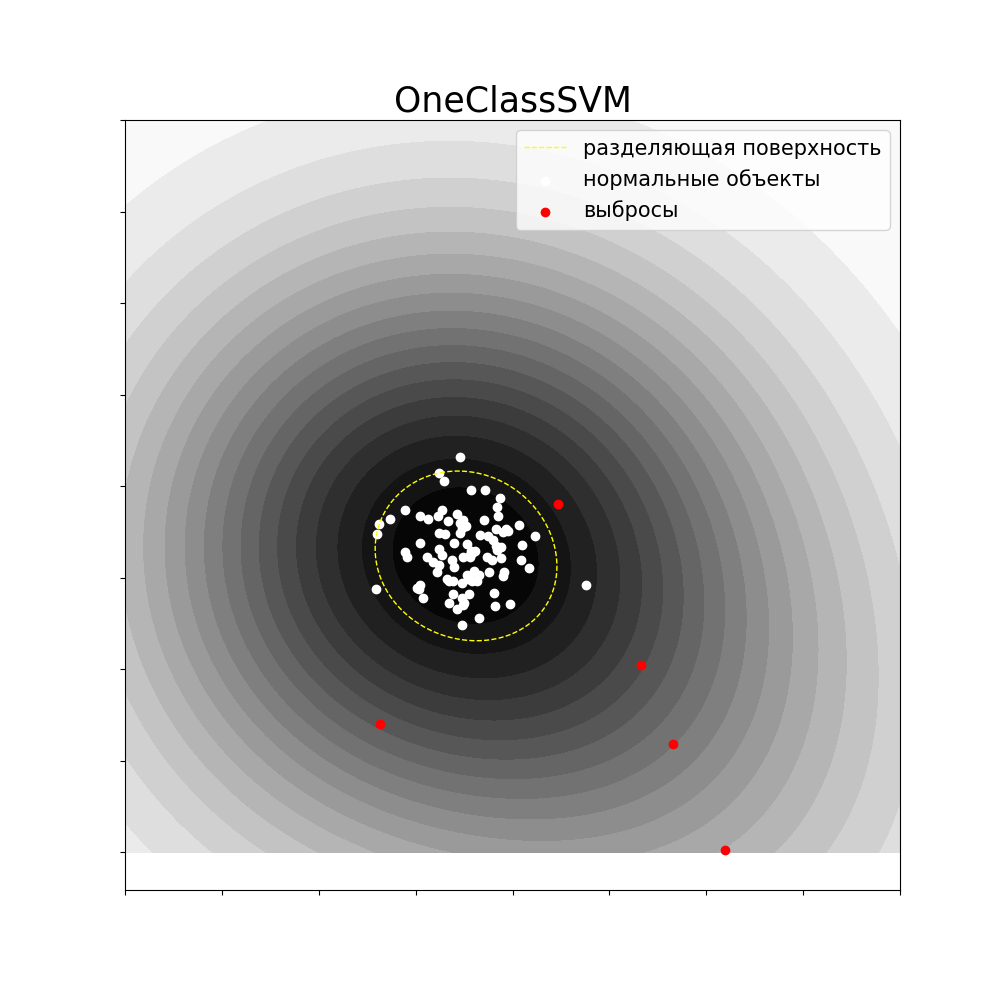
\includegraphics[width=0.3\linewidth]{OneClassSVM_1.png}
            \label{sec:Research:Model:Visualization:fig:OneClassSVM:1}
        }
        \subfigure[]{
            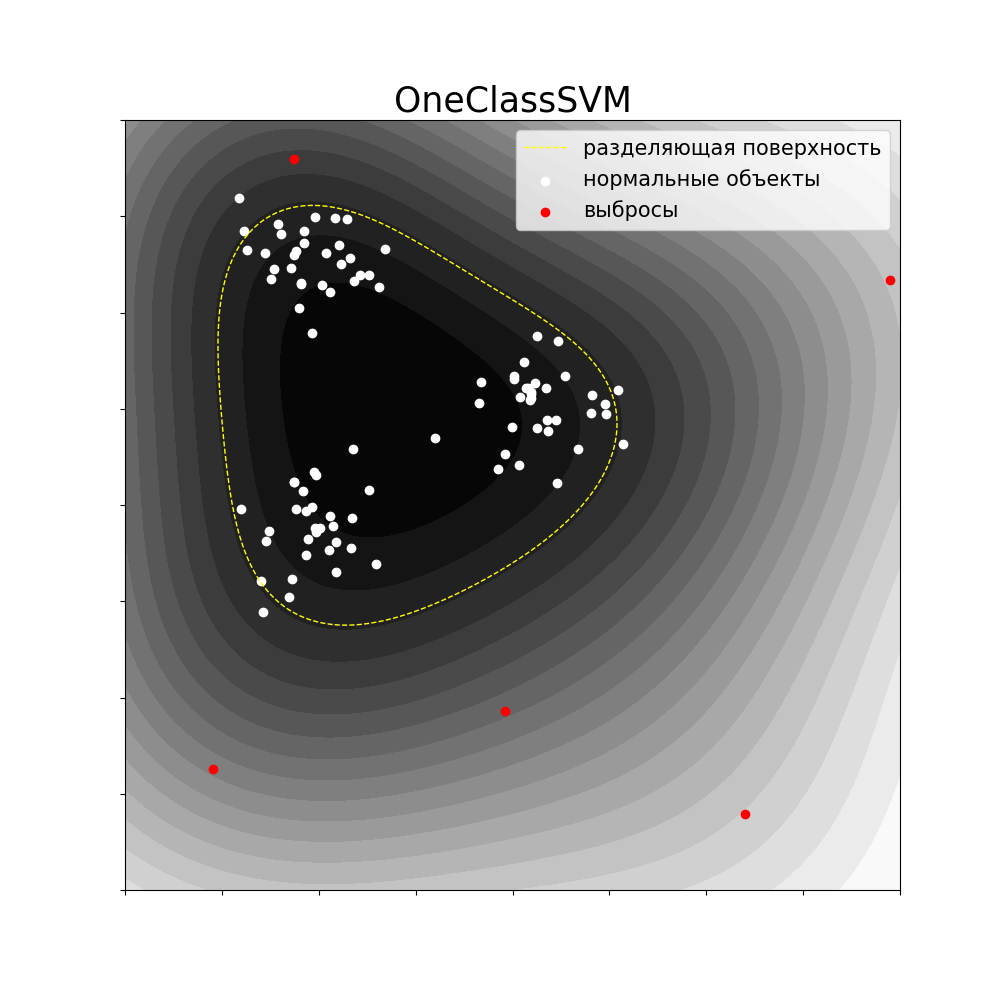
\includegraphics[width=0.3\linewidth]{OneClassSVM_3.png}
            \label{sec:Research:Model:Visualization:fig:OneClassSVM:3}
        }
        \subfigure[]{
            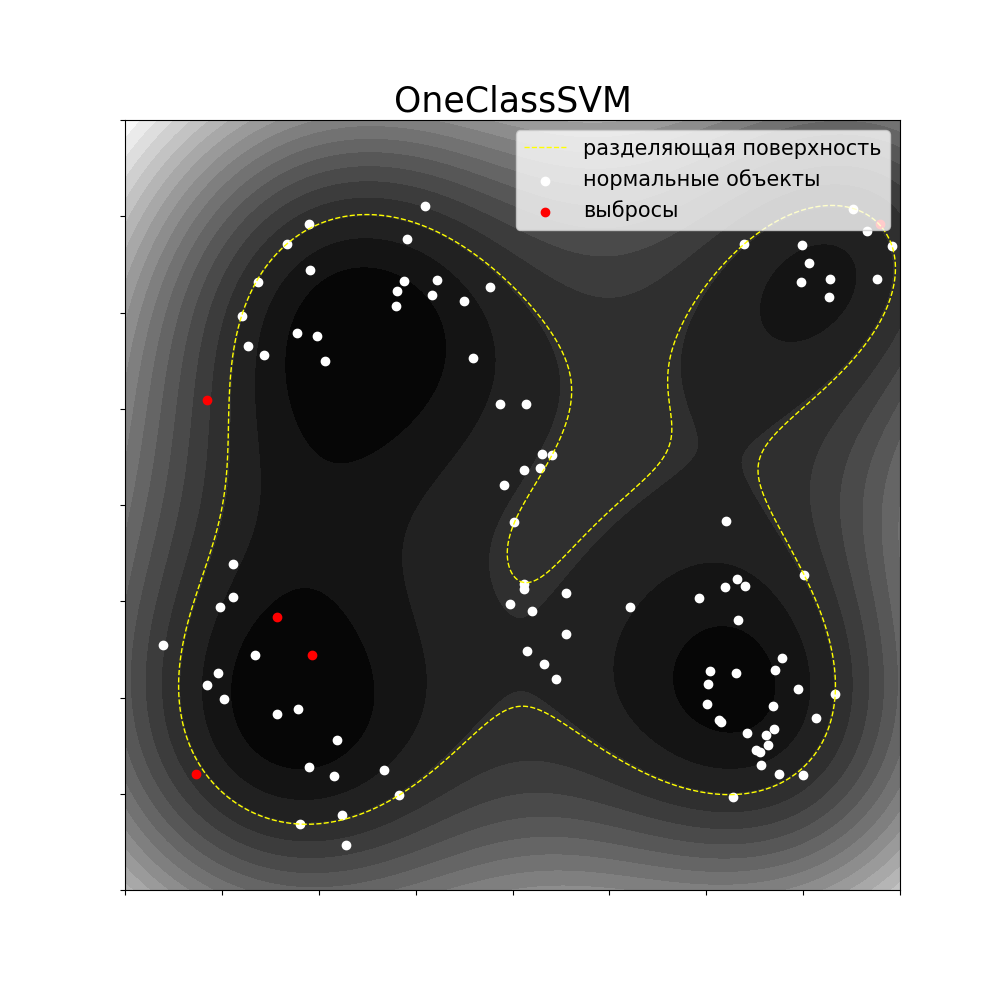
\includegraphics[width=0.3\linewidth]{OneClassSVM_10.png}
            \label{sec:Research:Model:Visualization:fig:OneClassSVM:10}
        }  
        \caption{ТОДО \subref{sec:Research:Model:Visualization:fig:OneClassSVM:1} }
        \label{sec:Research:Model:Visualization:fig:OneClassSVM}
    \end{figure}

    % IsolationForest
    \begin{figure}[h!]
        \centering
        \subfigure[]{
            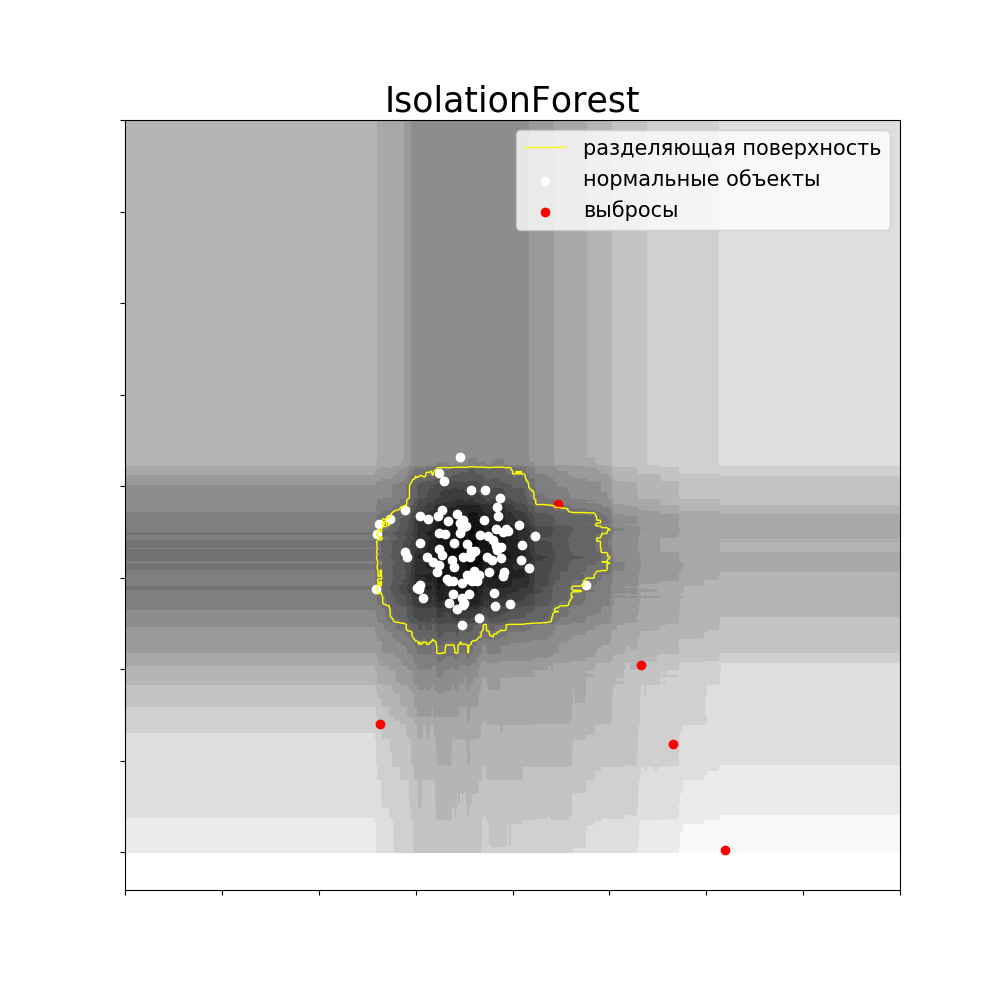
\includegraphics[width=0.3\linewidth]{IsolationForest_1.png}
            \label{sec:Research:Model:Visualization:fig:IsolationForest:1}
        }
        \subfigure[]{
            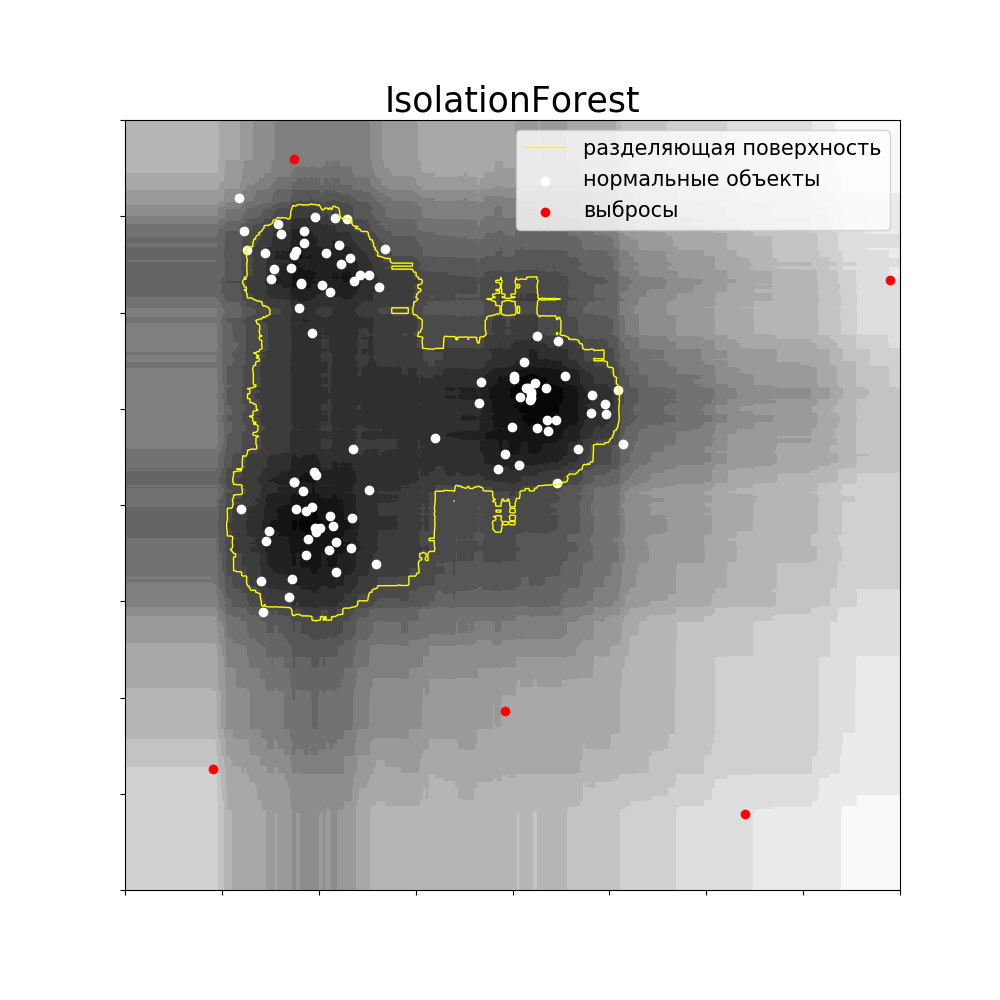
\includegraphics[width=0.3\linewidth]{IsolationForest_3.png}
            \label{sec:Research:Model:Visualization:fig:IsolationForest:3}
        }
        \subfigure[]{
            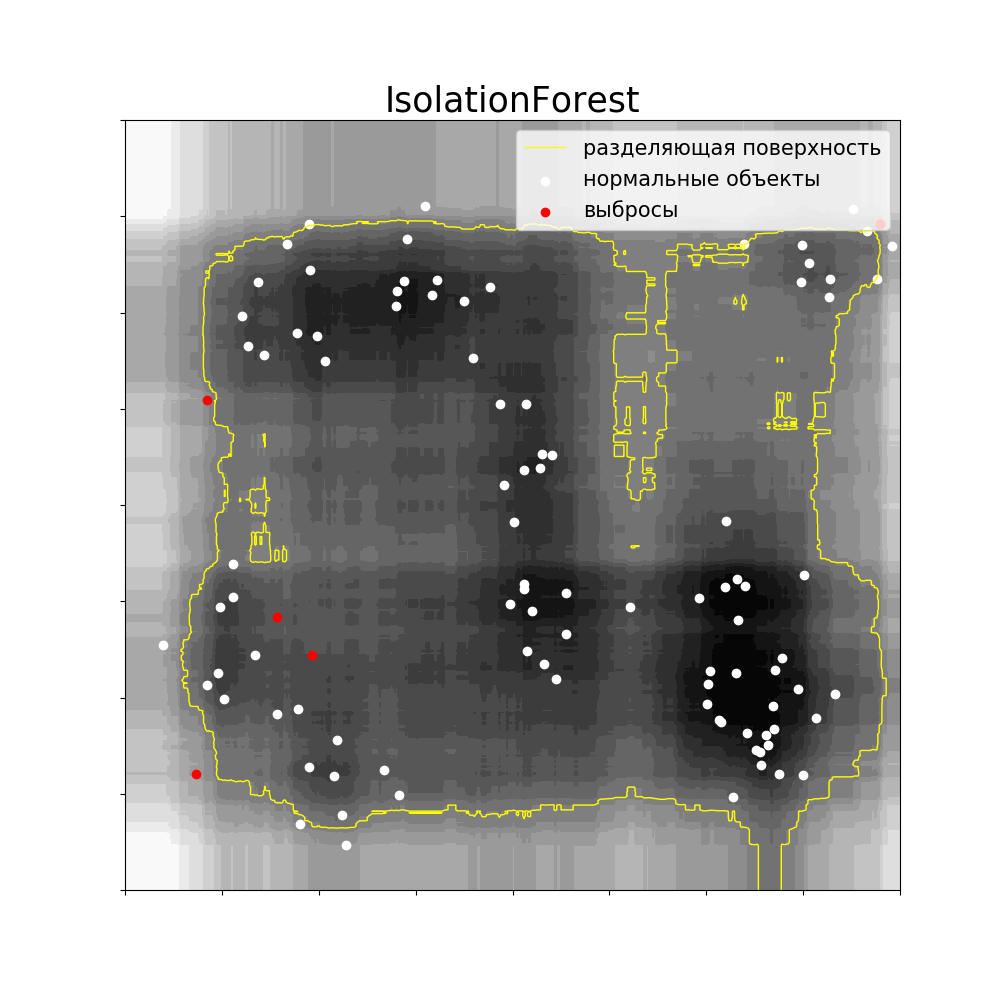
\includegraphics[width=0.3\linewidth]{IsolationForest_10.png}
            \label{sec:Research:Model:Visualization:fig:IsolationForest:10}
        }  
        \caption{ТОДО \subref{sec:Research:Model:Visualization:fig:IsolationForest:1}}
        \label{sec:Research:Model:Visualization:fig:IsolationForest}
    \end{figure}

    % EllipticEnvelope
    \begin{figure}[h!]
        \centering
        \subfigure[]{
            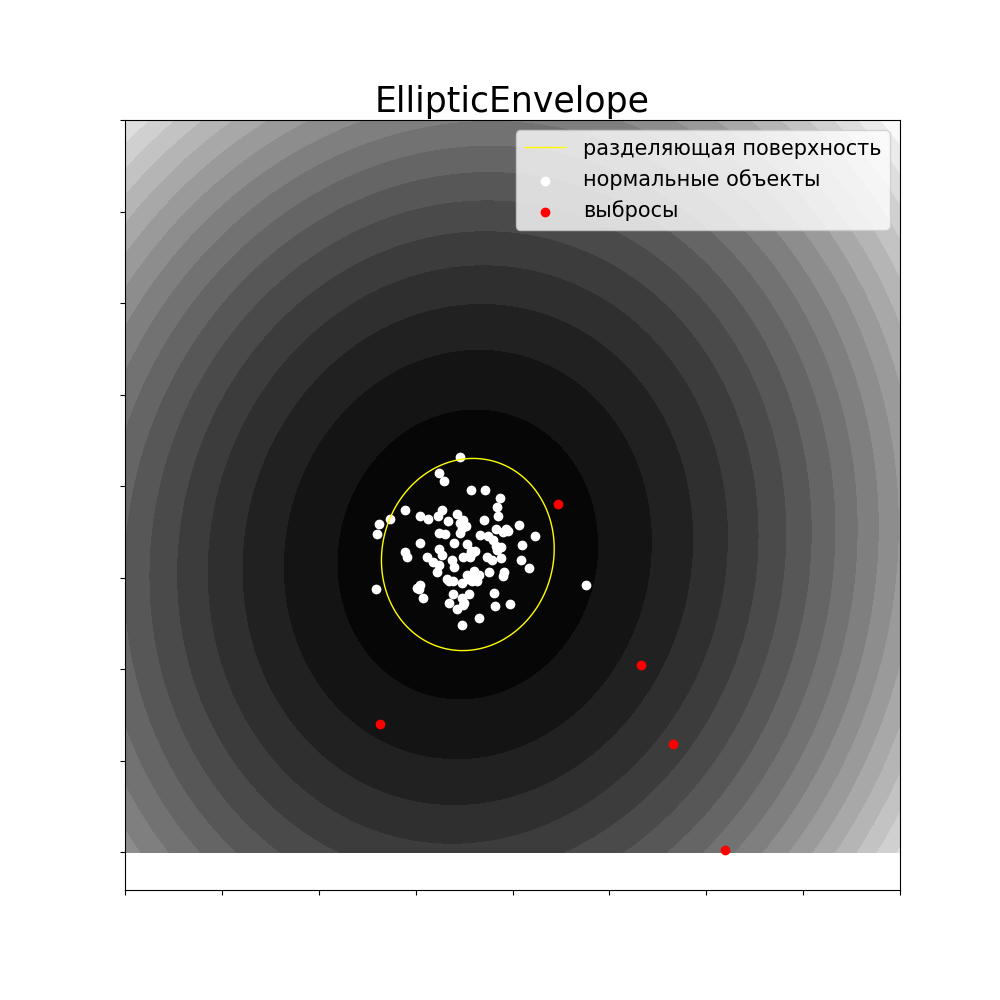
\includegraphics[width=0.3\linewidth]{EllipticEnvelope_1.png}
            \label{sec:Research:Model:Visualization:fig:EllipticEnvelope:1}
        }
        \subfigure[]{
            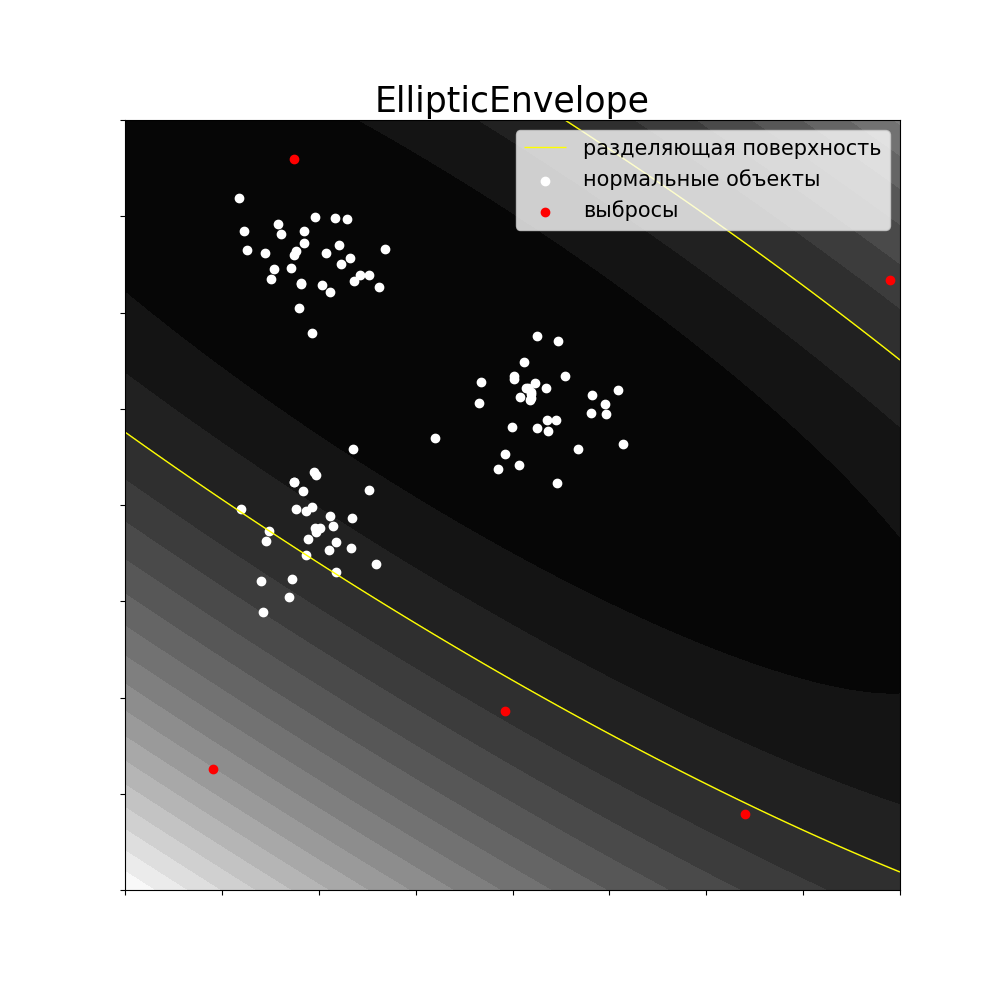
\includegraphics[width=0.3\linewidth]{EllipticEnvelope_3.png}
            \label{sec:Research:Model:Visualization:fig:EllipticEnvelope:3}
        }
        \subfigure[]{
            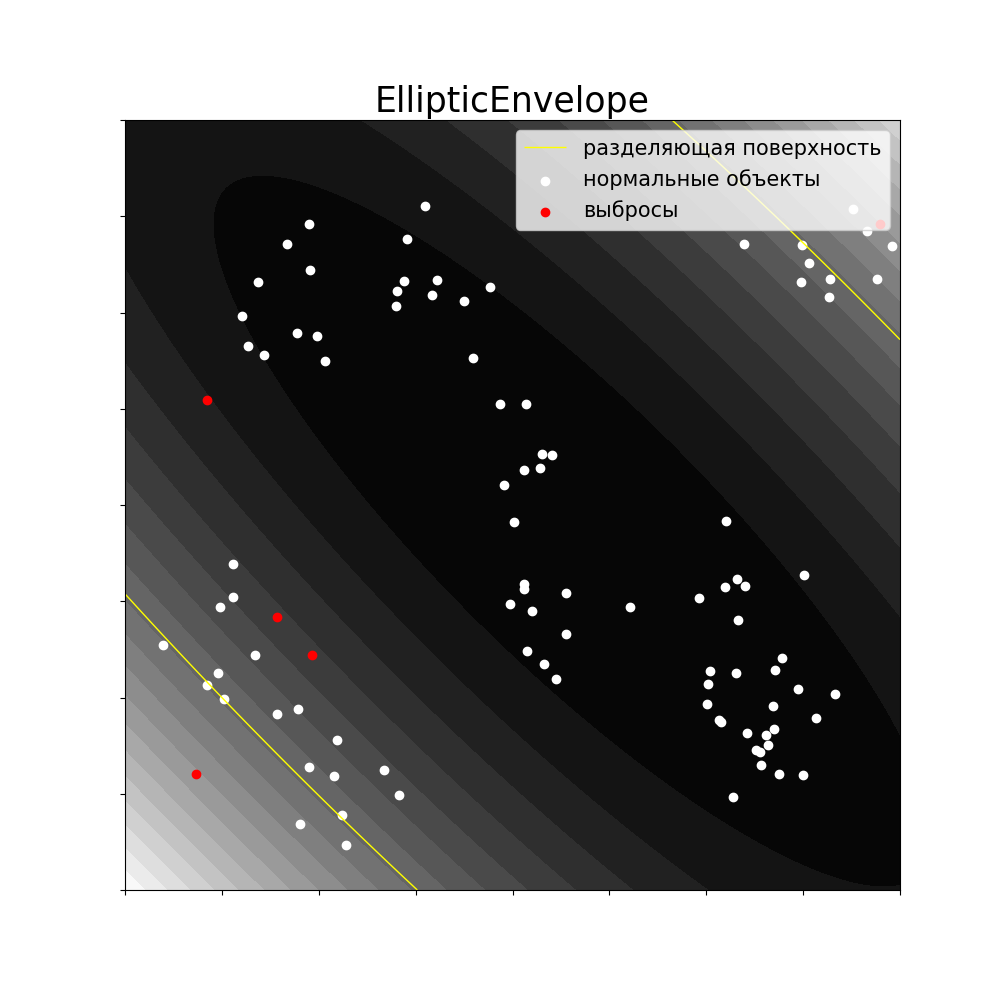
\includegraphics[width=0.3\linewidth]{EllipticEnvelope_10.png}
            \label{sec:Research:Model:Visualization:fig:EllipticEnvelope:10}
        }  
        \caption{ТОДО \subref{sec:Research:Model:Visualization:fig:EllipticEnvelope:1} }
        \label{sec:Research:Model:Visualization:fig:EllipticEnvelope}
    \end{figure}

    % LocalOutlierFactor
    \begin{figure}[h!]
        \centering
        \subfigure[]{
            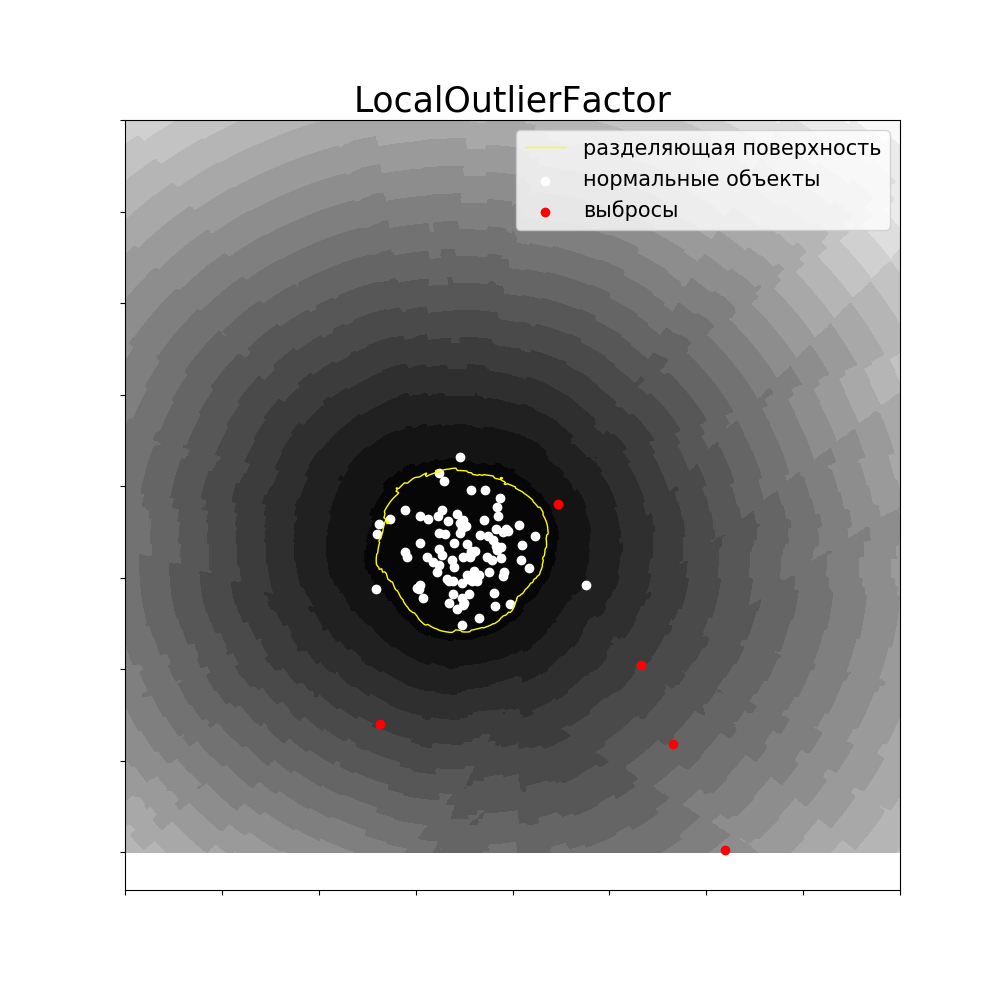
\includegraphics[width=0.3\linewidth]{LocalOutlierFactor_1.png}
            \label{sec:Research:Model:Visualization:fig:LocalOutlierFactor:1}
        }
        \subfigure[]{
            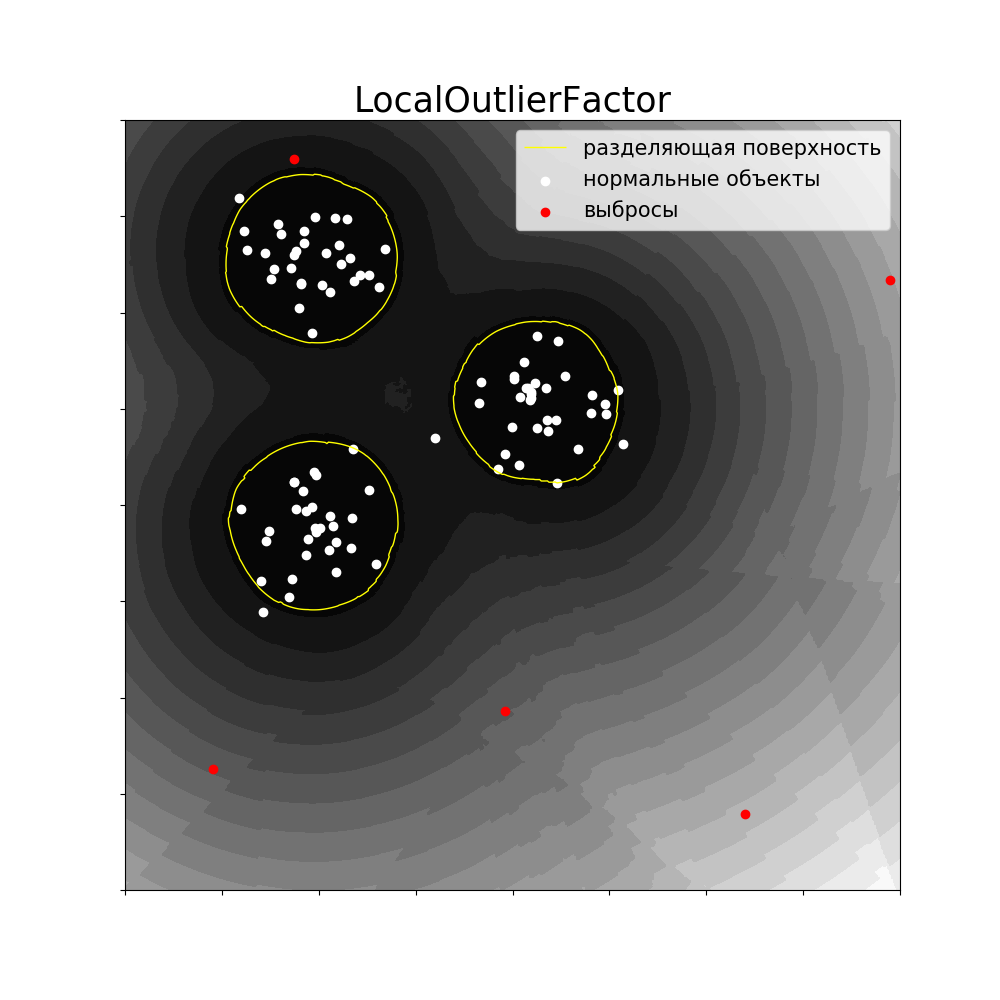
\includegraphics[width=0.3\linewidth]{LocalOutlierFactor_3.png}
            \label{sec:Research:Model:Visualization:fig:LocalOutlierFactor:3}
        }
        \subfigure[]{
            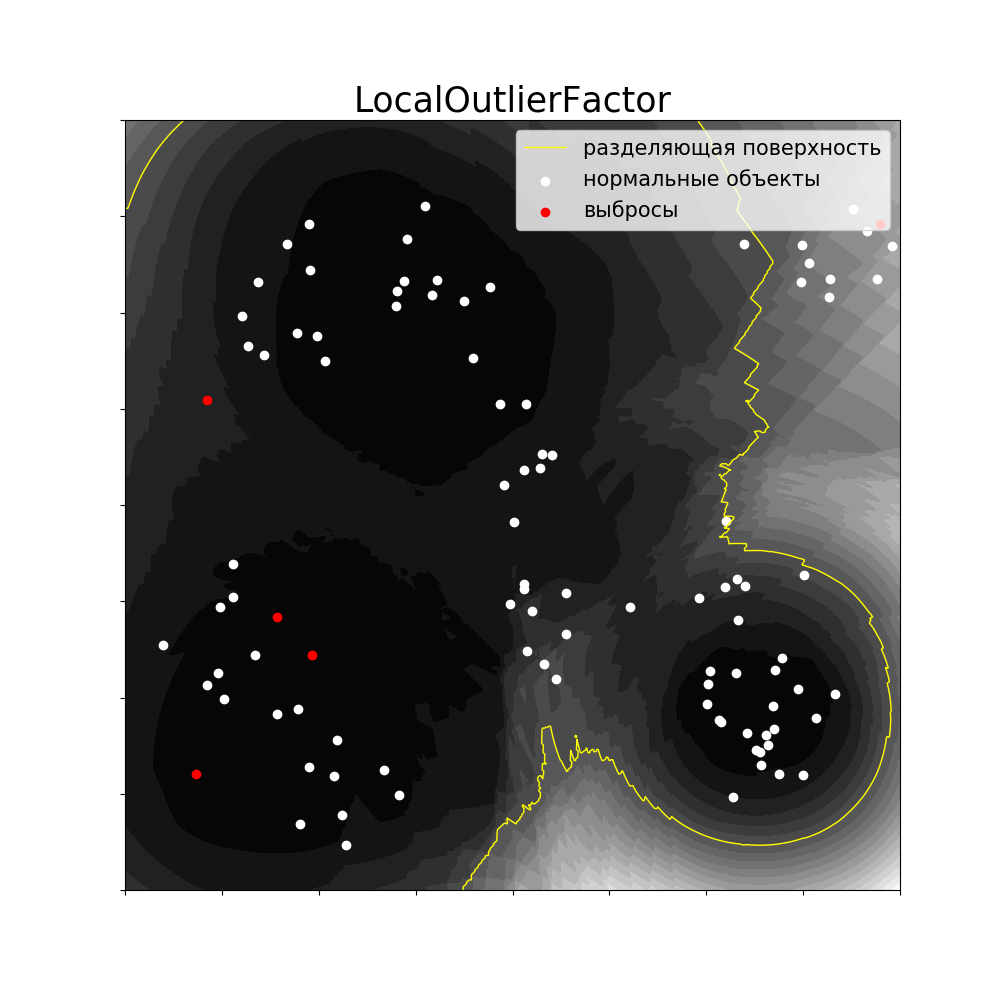
\includegraphics[width=0.3\linewidth]{LocalOutlierFactor_10.png}
            \label{sec:Research:Model:Visualization:fig:LocalOutlierFactor:10}
        }  
        \caption{ТОДО \subref{sec:Research:Model:Visualization:fig:LocalOutlierFactor:1} }
        \label{sec:Research:Model:Visualization:fig:LocalOutlierFactor}
    \end{figure}


    \newpage



    \section{Описание практической части}
    \label{sec:PracticalPart}

    \newpage



    \section{Планы на будущее}
    \label{sec:Future}

    \newpage



    \section{Заключение}
    \label{sec:Conclusion}

    \newpage



    \begin{thebibliography}{20}
        \bibitem{1}
        Jain A. K., Ross A., Prabhakar S. An introduction to biometric recognition //IEEE Transactions on circuits and systems for video technology. – 2004. – Т. 14. – №. 1. – С. 4-20.

        \bibitem{2}
        https://www.johndcook.com/blog/2018/10/31/biometric-security-error/

        \bibitem{BALABIT}
        Fülöp, Á., Kovács, L., Kurics, T., Windhager-Pokol, E. (2016). Balabit Mouse Dynamics Challenge data set. Available at: https://github.com/balabit/Mouse-Dynamics-Challenge

        \bibitem{TWOS}
        Harilal A. et al. Twos: A dataset of malicious insider threat behavior based on a gamified competition //Proceedings of the 2017 International Workshop on Managing Insider Security Threats. – 2017. – С. 45-56.
        
        \bibitem{Dyakonov}
        https://dyakonov.org/2017/04/19/поиск-аномалий-anomaly-detection/
        
        \bibitem{NoveltyDetection}
        Pimentel M. A. F. et al. A review of novelty detection //Signal Processing. – 2014. – Т. 99. – С. 215-249.
        
        \bibitem{IsolationForest}
        Liu F. T., Ting K. M., Zhou Z. H. Isolation forest //2008 Eighth IEEE International Conference on Data Mining. – IEEE, 2008. – С. 413-422.
        
        \bibitem{IsolationForest_2}
        https://towardsdatascience.com/outlier-detection-with-isolation-forest-3d190448d45e
        
        \bibitem{IsolationForeset_3}
        https://towardsdatascience.com/anomaly-detection-with-isolation-forest-visualization-23cd75c281e2

        \bibitem{3}
        Mondal S., Bours P. A study on continuous authentication using a combination of keystroke and mouse biometrics //Neurocomputing. – 2017. – Т. 230. – С. 1-22.

        \bibitem{4}
        Feher C. et al. User identity verification via mouse dynamics //Information Sciences. – 2012. – Т. 201. – С. 19-36.
        
    \end{thebibliography}


\end{document}
